% !TEX TS-program = xelatex
% !TEX encoding = UTF-8 Unicode

\documentclass[AutoFakeBold]{LZUThesis}
\usepackage{wasysym}
\usepackage{enumitem}
\usepackage[most]{tcolorbox}
\usepackage{multirow}
\usepackage{tikz}
\usetikzlibrary{arrows.meta, decorations.markings}
\usepackage{hyperref}
\usepackage[numbers,sort&compress]{natbib}
\newcommand{\upcite}[1]{\textsuperscript{\textsuperscript{\cite{#1}}}}
\allowdisplaybreaks[4]

\begin{document}

\title{{果蝇的多因子综合遗传分析}}

\entitle{{Multifactorial Comprehensive Genetic Analysis of \textit{Drosophila melanogaster}}}

\author{生物信息学班 李泽华 320210928501}
\major{遗传学}
\advisor{王铭裕}
\college{生命科学学院}
\grade{2021级}


\frontmatter

\ZhAbstract{
本研究通过果蝇的多因子综合遗传分析,探究了基因的分离定律, 自由组合定律, 伴性遗传规律和连锁交换定律。
实验中,利用$F_2$代体色数据,对F2代各个数据与预期数值进行卡方检验,研究了正交、
反交和正反交比较的自由度、卡方值和P值, 验证了各个遗传定理。同时,确定了基因位点的顺序
为体色, 翅型, 眼色, 并完成了基因作图.
实验结果为深入理解果蝇遗传特性提供了重要线索。
}{果蝇
,多因子综合遗传分析
,分离定律
,自由组合定律
,伴性遗传规律
,连锁交换定律
,遗传定理
,基因位点
,基因作图}

\EnAbstract{
This study employs a multifactorial genetic analysis of fruit flies to investigate 
the laws of gene segregation, independent assortment, co-inheritance, and linkage exchange.
In the experiment, chi-square tests were conducted on the F2 generation body color data to 
examine the degrees of freedom, chi-square values, and P values for orthogonal, reciprocal, 
and reciprocal comparison. This validated various genetic principles. Simultaneously, 
the order of gene loci was determined as body color, wing type, and eye color, 
and genetic mapping was completed. The experimental results offer vital insights for a 
thorough understanding of the genetic characteristics of fruit flies.
}{Fruit fly
,Multifactorial genetic analysis
,Law of segregation
,Law of independent assortment
,Law of co-inheritance
,Law of linkage exchange
,Genetic principles
,Gene loci
,Genetic mapping}

\customcontent

\mainmatter

\chapter{\texorpdfstring{绪 \quad 论}{绪论}}
多因子遗传分析是遗传学领域中的一项关键研究,旨在理解基因如何相互作用以影响生物体的性状。果蝇(Drosophila melanogaster)作为经典的模式生物,在遗传学研究中发挥着重要的作用。通过对果蝇进行综合的遗传分析,我们可以深入了解不同基因之间的关系,揭示其对性状表现的影响。

本研究聚焦于果蝇的多因子遗传,特别关注了体色、翅型、眼色、刚毛等性状。这些性状的综合研究有助于我们更全面地认识基因之间的相互作用,以及它们在遗传传递中的规律。此外,通过正交和反交的交叉分析,我们试图z验证遗传学定律, 揭示基因的连锁交换定律,深入挖掘基因在遗传过程中的转换规律。

在遗传学的发展历程中,早期的科学家们,如孟德尔(Mendel)、摩根(Morgan)等,为我们奠定了遗传学的基石。然而,随着科技的发展,对于多基因性状的理解仍然面临诸多挑战。

通过本论文的深入分析,我们期望能够为果蝇遗传学研究贡献新的数据,同时为多因子遗传分析提供实质性的研究成果。这对于理解其他生物体的遗传特性,以及在医学和农业等领域的应用,都具有重要的指导意义。

因此,本研究旨在通过果蝇的多因子遗传分析,深化我们对基因相互作用和连锁交换定律的认识,为遗传学领域的进一步研究提供坚实的基础。
\chapter{研究背景}
\section{遗传学三大定律}
\begin{enumerate}
\item 分离定律\par
\hspace{2em}分离定律\upcite{mendel1996}又称为孟德尔第一定律。控制相对性状的一对等位基因在杂合于中各自保持其独立性、在配子形成时,彼此分开,随机地进入不同的配子中。在止常情况下,P,
杂合子的配子分离比为1:1,F代的基因型分离比是1:2:1(如图\ref{fig:1})。如果相对性状间呈完全显性关系,则具有一对相对性状差异的两纯合亲本杂交,F杂合子表现显性性状,其测
交子代(即F杂合子与隐性纯合亲本回交的子代)和自交子代(F)都只有显性和隐性两种表型,前者比例为1:1;后者比例为3:1。如果相对性状间呈不完全显性或并显
性,则F,表现两亲本的中间性状,其测交和自交子代表型分离比就等同于基因型分离比。因此可以根据杂交的配子类型及比例、$F_1$、$F_2$以及测交子代群体表型类型与比例等
对相对性状进行遗传分析。
\end{enumerate}

\begin{figure}[htbp]
    \centering
    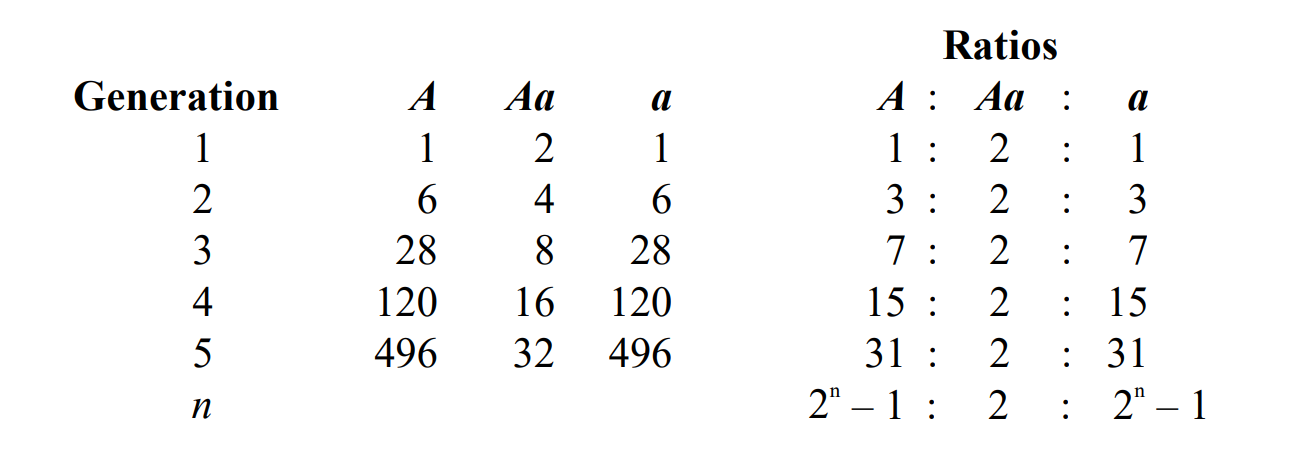
\includegraphics[width=1.1\textwidth]{img/mendel}
    \caption{孟德尔对杂交实验的分析\upcite{mendel1996}}
    \label{fig:1}
\end{figure}

\begin{enumerate}[start=2]
\item 自由组合定律\par
\hspace{2em}自由组合定律\upcite{mendel1996}又称为独立分配定律(Law of Independent Assortment)或孟德尔第二定律。支配两对(或两对以上)不同性状的等位基因,在杂合状态保持其独立性。配子形
成时,各等位基因彼此独立分离,不同对的基因自由组合。在一般情况下,$F_1$配子分离比为1:1:1:1;$F_2$基因型分离比率为$(1:2:1)^2$,即$(1/4+2/4+1/4)^2$三项式展开式
的各项系数;显性完全时,$F_2$表型比率为$(3:1)^2$, 即 $(3/4 + 1/4)^2$ 二项式展开式的各项系数 (9:3:3:1). 
因此可以根据杂交的配子类型及比例, $F_1$代, $F_2$代群体表型类型及
比例等对两对(或两对以上)相对性状的分离和组合进行遗传分析(如图\ref{fig:2})。

\begin{figure}[h]
    \centering
    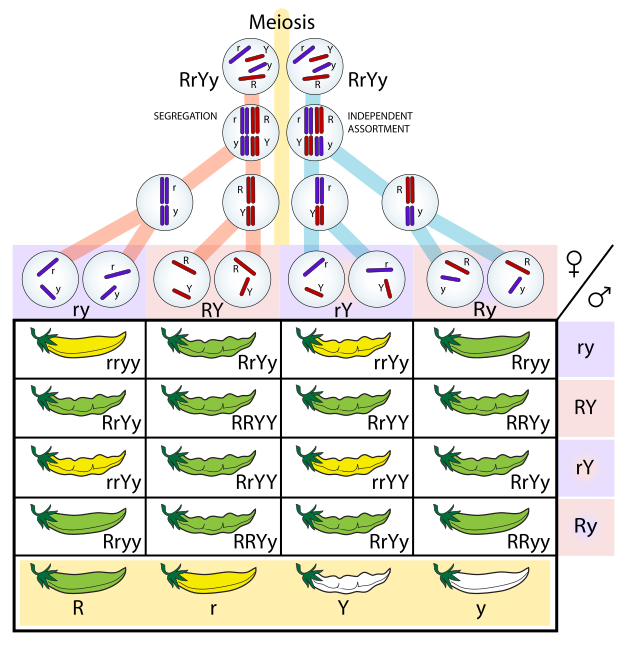
\includegraphics[width=0.4\textwidth]{img/Independent_assortment_&_segregation}
    \caption{孟德尔的自由组合实验\upcite{wiki:mendelimg}}
    \label{fig:2}
\end{figure}

\item 连锁定律\par
\hspace{2em}连锁定律\upcite{morgan1917}又称为孟德尔第三定律。支配同一染色体上的等位基因,在杂合状态下,由于连锁作用,两个等位基因彼此连锁在一起,不能分离。在减数分裂时,两个连锁的等位基因
必须同时进入同一配子中。因此,连锁基因的分离比率小于1:1,而是接近于1:1。连锁基因的分离比率越小,连锁越紧密。连锁基因的分离比率可以用连锁值来表示。连锁值
越大,连锁越松弛;连锁值越小,连锁越紧密。连锁值的计算公式为:连锁值= (重组子代数/总子代数)$\times 100\%$。连锁值的计算方法有两种:一是根据杂交的配子类型及比例, $F_1$代,
$F_2$代群体表型类型及比例等进行遗传分析,计算连锁值;二是根据连锁基因的遗传连锁图,计算连锁值。连锁值的计算方法有两种:一是根据杂交的配子类型及比例, $F_1$代,

\end{enumerate}
\section{伴性遗传}
生物某些性状的溃传常与性别联系在一杞,这种现象称为伴性遗传或性连锁遗传(sex-linkedinheritance)\upcite{morgen-sexlinkage}这是由于支配其性状的基因位于性染色体上。性染色体是指
直接与性别有关的一对或一个染色体. 拥有一对同型性染色体的个体统称为同配性别,具有一对异型性染色体的个休则称为异配性别。果蝇属XY型性别决定的生物, 通常情况下, 雌果蝇的性染色体构成为XX,雄果帷的性染色体构成为XY.
伴性遗传可以归纳为下列两条遗传规律:\par
\begin{enumerate}
\item 当同配性别传弟纯合显性基因时, $F_1$代雌、雄个体都为显性性状。$F_2$代性状的分离呈3显性:1隐性;性别的分离呈1:1, 其中隐性个体的性别与祖代隐性个体一样, 即外祖父的性状传递给1/2外孙。\par
\item 当同配性别传递纯合隐性基因时,$F_1$代表现交叉遗传,即母亲的性状传给儿子, 父亲的性状传给女儿。$F_2$代性状与性别的比均为1:1。\par
\end{enumerate}

\begin{figure}[hbtp]
    \centering
    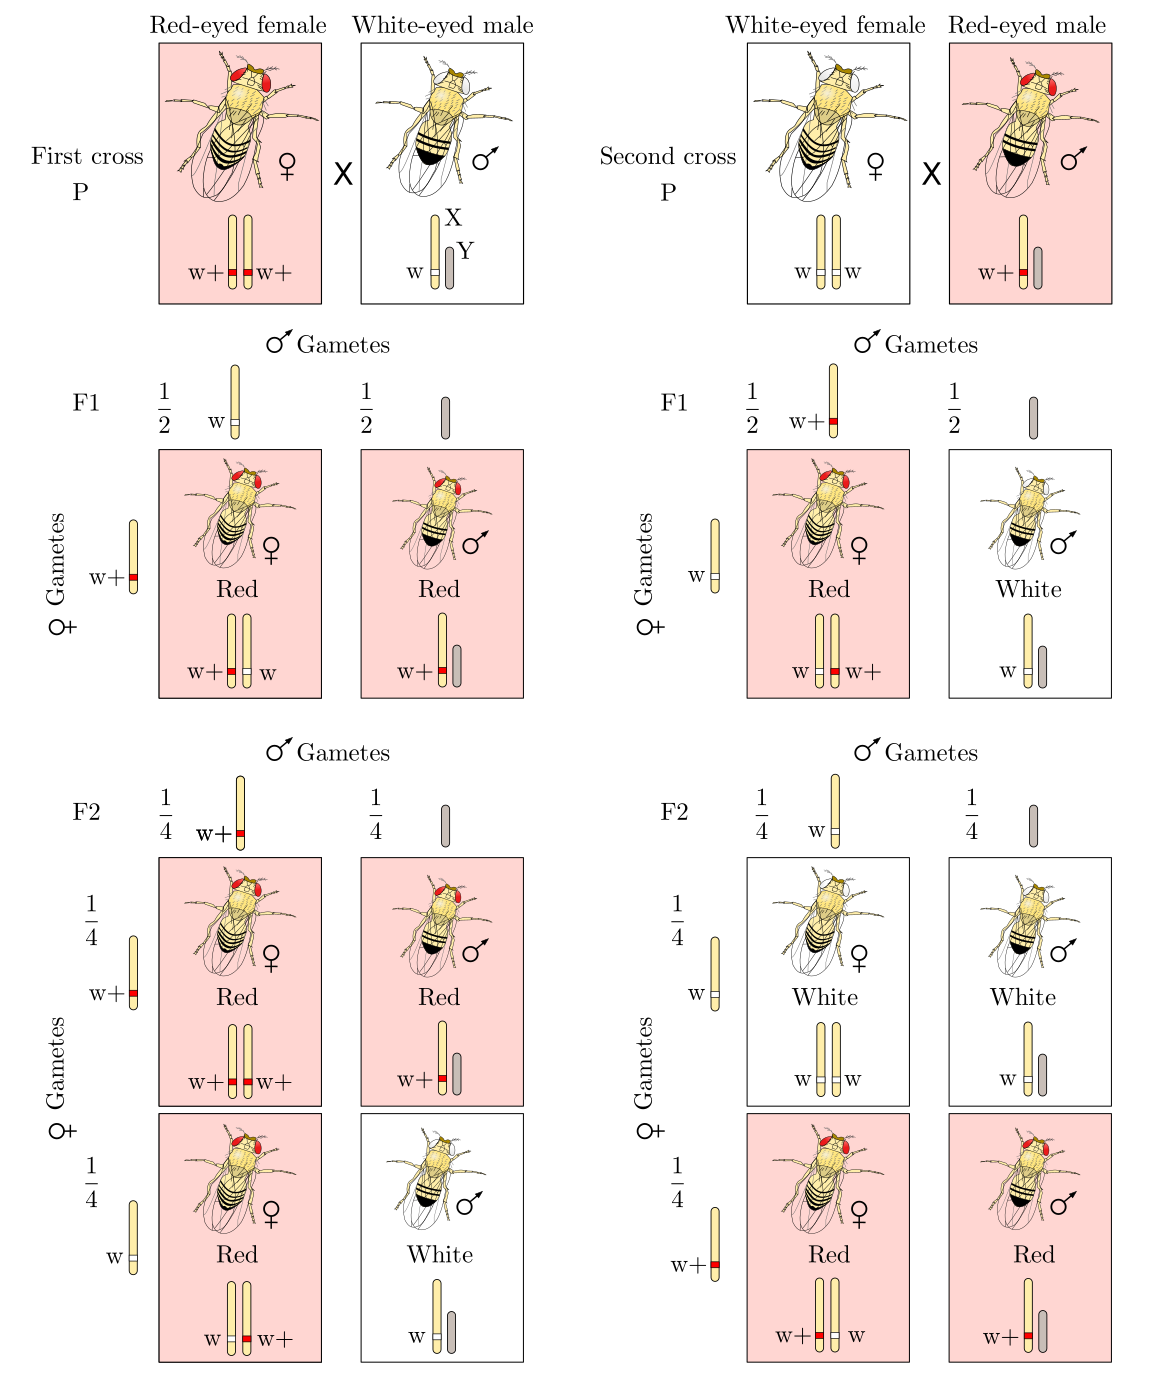
\includegraphics[width=0.35\textwidth]{img/Sex-linked_inheritance}
    \caption{摩尔根的果蝇杂交实验\upcite{sex-linked-inheritance}}
    \label{fig:3}
\end{figure}

\indent 果蝇的红眼和白眼是一对相对性状, 控制该对性状的基因位于X染色体上,在Y染色体没有与之对应的等位基因, 且红眼($X^+$)对白眼$(X^w$)为完全显性。将红眼果蝇和白眼果蝇杂交,其后代眼色的表现与性别相关,而且正反交的结果不同。\par

\chapter{研究目的与方法}

\section{研究目的}
\begin{itemize}
    \item 掌握果蝇的杂交技术和实验数据的统计处理方法
    \item 通过一次涉及多因子的果蝇杂交实验, 同时检验遗传的三大定律以及伴性遗传的规律
    \item 在掌握基因分离, 自由组合, 连锁与交换的遗传分析方法的同时, 从纷繁复杂的现象中找出遗传规律及其内在的联系
    \item 培养运用所学的遗传学知识, 综合判断, 分析和解决问题的能力
\end{itemize}

\section{研究方法}
\subsection{实验材料与数据获取}
\begin{itemize}
    \item 实验材料\par
黑腹果蝇的野生品系(红眼, 直刚毛, 长翅, +++//+++, +++//Y)\par
三隐品系(白眼, 焦刚毛, 小翅, w sn m//w sn m, w sn m//Y)
    \item 实验试剂\par
乙醚, 乙醇, 丙酸, 蒸馏水, 琼脂粉, 玉米粉, 酵母粉, 蔗糖, 红糖
    \item 器材\par
恒温培养箱, 双目解剖镜, 高压灭菌锅, 电子天平, 白瓷版, 镊子, 毛笔, 解剖针, 培养瓶
\end{itemize}
\subsection{实验步骤}
\begin{enumerate}
    \item 原种果蝇培养\par
    \hspace{2em}于杂交实验开始前两周,\SI{20}{\degreeCelsius}条件下分别培养长翅和残翅果蝇品系。待每个培养瓶幼虫化蛹之后,移去培养瓶中的成蝇,准备从羽化不超过12h的果蝇中挑选杂交亲本。
    \item 挑选杂交亲本果蝇\par
    \hspace{2em}选长翅和残翅果蝇为亲本,做正交和反交组合。由于雌蝇生殖器官中有贮精囊,一次交配可保留大量精子,供多次排卵受精用,因此做杂交实验前必须收集未交配过的处女蝇。刚羽化的雌蝇在12h内一般无交配能力,因此在杂交实验开始前放出亲本培养瓶中的所有成蝇,然后每隔10-12h收集一次刚羽化出的成蝇,
    并将雌雄蝇分开饲养。收
    集处女蝇数量的多少根据需要而定,通常不少于5对。
    \item 麻醉接种\par
    \hspace{2em}用长翅果蝇与残翅果蝇杂交,正反交同时进行。即长翅\female $\times$残翅\male,残翅\female $\times$长翅\male。将所选处女蝇按品系分别麻醉,按不同杂交组合分别选取雌、雄果蝇各6-10只移入杂交瓶中,为了防止昏迷果蝇被培养基粘住,可将培养瓶放倒,将果蝇置于瓶壁,待其完全苏醒后再将培养瓶直立,贴上标签。标明杂交亲本、杂交日期、实验人姓名。将杂交瓶放在\SI{25}{\degreeCelsius}恒温箱内培养。\par
    \vspace{0.25cm}
    \begin{minipage}{0.45\textwidth}
        \begin{tcolorbox}[colback=blue!10!white,colframe=blue!50!black,title=标签 1]
            \begin{center}
                \female 长翅(+//+) $\times$ \male 残翅(vg//vg)\par
            \end{center}
            日期: \par
            姓名: \par
        \end{tcolorbox}
    \end{minipage}%
    \hfill
    \begin{minipage}{0.45\textwidth}
        \begin{tcolorbox}[colback=green!10!white,colframe=green!50!black,title=标签 2]
            \begin{center}
                \female 残翅(vg//vg) $\times$ \male 长翅(+//+)\par
            \end{center}
            日期: \par
            姓名: \par
        \end{tcolorbox}
    \end{minipage}
    \vspace{0.25cm}

    \item 去亲本\par
    \hspace{2em}杂交培养7d后、亲本果帆都已杂交产卵。在杂种幼虫化蛹羽化前,将亲本移出弃去,目的是防止亲本与$F_1$代成蝇发生回交(移去的果蝇最好处死)。
    \item 观察杂种$F_1$代\par
    \hspace{2em}继续培养7d,$F_1$代果蝇羽化为成虫后,经麻醉在白瓷板上用解剖镜观察和统计正反交$F_1$代个体的性状,判断$F_1$代个体的性状是否和预期结果一致。
    \item 观察杂种$F_2$代\par
    \hspace{2em}分别收集正反交$F_1$代果蝇6-10对放入一新培养瓶,在\SI{25}{\degreeCelsius}恒温箱内继续培养7d后,移去$F_1$代果蝇。再培养7d,$F_2$代成蝇出现,观察并统计$F_2$代的性状表现类型及数目。并将观察结果填入记录表。
    \item 统计检验\par
    \hspace{2em}用$x^2$检验法对试验结果进行统计检验,验证分离定律, 自由组合定律, 连锁定律和伴性遗传规律。
\end{enumerate}

\chapter{实验结果与分析}
\section{实验数据结果汇总}

\begin{longtable}{cccccc}
    \label{tab:1}
    \caption{正交$F_1$代和$F_2$代观察记录表}\\
    \toprule
    \multirow{2}{*}{正交} & \multicolumn{2}{c}{\female} & \multicolumn{2}{c}{\male} & \multirow{2}{*}{合计} \\
    \cmidrule(lr){2-5}
    & 性状 & 数量 & 性状 & 数量 & \\
    \midrule
    P       & 灰白焦小  &       & 灰红直长  &       &       \\
    $F_1$   & 灰红直长  & 1618  & 灰白焦小  & 1355  & 2973  \\
    \midrule
    \multirow{2}{*}{$F_2$} & \multicolumn{2}{c}{灰体} & \multicolumn{2}{c}{黑体} & \\
    \cmidrule(lr){2-6}
    & \female & \male & \female & \male & \\
    \midrule
    红直长($+ + +$)     & 1509  & 1122  & 458   & 339   & 3428 \\
    白焦小($w sn m$)    & 1059  & 959   & 298   & 259   & 2611 \\
    白直长($w + +$)     & 252   & 211   & 70    & 68	& 601  \\
    红焦小($+ sn m$)    & 186   & 181   & 70    & 54	& 491  \\
    红直小($+ + m$)     & 283   & 251   & 99    & 84	& 717  \\
    白焦长($w sn +$)    & 292   & 218   & 74    & 100   & 684  \\
    红焦长($+ sn +$)    & 91    & 73    & 29    & 21	& 214  \\
    白直小($w + m$)     & 90    & 67    & 26    & 29	& 212  \\
    体色合计 & \multicolumn{2}{c}{6744} & \multicolumn{2}{c}{2078} & \\
    性别合计 &  3762 & 2982 & 1124 & 954 & \\
    \midrule
    性别合计 & \female & 4886 & \male & 3936 &  \\
    \bottomrule
\end{longtable}


\begin{longtable}{cccccc}
    \label{tab:2}
    \caption{反交$F_1$代和$F_2$代观察记录表}\\
    \toprule
    \multirow{2}{*}{反交} & \multicolumn{2}{c}{\female} & \multicolumn{2}{c}{\male} & \multirow{2}{*}{合计} \\
    \cmidrule(lr){2-5}
    & 性状 & 数量 & 性状 & 数量 & \\
    \midrule
    P       & 灰红直长  &       & 灰白焦小  &       &       \\
    $F_1$   & 灰红直长  & 3223  & 灰红直长  & 3156  & 6379  \\
    \midrule
    \multirow{2}{*}{$F_2$} & \multicolumn{2}{c}{灰体} & \multicolumn{2}{c}{黑体} & \\
    \cmidrule(lr){2-6}
    & \female & \male & \female & \male & \\
    \midrule
    红直长($+ + +$)     & 1884 & 506 & 513   &   185   & 3800 \\
    白焦小($w sn m$)    & 46   & 422 & 36	 &   161   & 665  \\
    白直长($w + +$)     & 13   & 97	 & 13	 &   31	   & 154  \\
    红焦小($+ sn m$)    & 21   & 109 & 18	 &   28	   & 176  \\
    红直小($+ + m$)     & 70   & 104 & 34	 &   50	   & 258  \\
    白焦长($w sn +$)    & 35   & 120 & 7	 &   20	   & 182  \\
    红焦长($+ sn +$)    & 65   & 30	 & 24	 &   21	   & 140  \\
    白直小($w + m$)     & 12   & 20	 & 12	 &   9	   & 53   \\
    体色合计 & \multicolumn{2}{c}{3554} & \multicolumn{2}{c}{1162} & \\
    性别合计 & 2146 & 1408 & 657 & 505 & \\
    \midrule
    性别合计 & \female & 2803 & \male & 1913 &  \\
    \bottomrule
\end{longtable}

\section{实验结果分析}
\subsection{$F_1$代正反交数据分析}
根据表\ref{tab:1}和表\ref{tab:2}中表型的数量, 与预期比例$3:1$对应的预期值进行卡平方检验(具体分析过程见附录), 得到结果如下:

\begin{table}[htbp]
    \centering
    \caption{$F_1$代正反交数据卡方检验结果}
    \begin{tabular}{cccc}
        \toprule
        杂交组合 & 自由度 & 卡方值 & P值 \\
        \midrule
        正交 & 1 & 11.479067341269548 & 0.000703844419500476 \\
        反交 & 1 & 0.33117389293543964 & 0.5649686736181281 \\
        \bottomrule
    \end{tabular}
    \label{tab:3}
\end{table}

从表\ref{tab:3}中可以看出, 正交组合的P值小于0.05, 反交组合的P值大于0.05, 因此从正交的数据中我们的观测值与预期值之间差异显著, 不能认为符合$3:1$的分离比例, 而反交的数据中我们的观测值与预期值之间差异不显著, 可以认为符合$3:1$的分离比例。

\subsection{$F_2$代正反交数据分析}

\subsubsection{基因的分离定律}
以体色为对象, 研究果蝇$F_2$代的分离比例。根据表\ref{tab:1}和表\ref{tab:2}中体色的数量, 与预期比例$3:1$对应的预期值以及正反交之间进行卡平方检验(具体分析过程见附录), 得到结果如下:

\begin{table}[htbp]
    \centering
    \caption{$F_2$代体色数据卡方检验结果}
    \begin{tabular}{cccc}
        \toprule
        杂交组合 & 自由度 & 卡方值 & P值 \\
        \midrule
        正交 & 1 & 7.860818618252946 & 0.005051751529436341 \\
        反交 & 1 & 0.14545707776087888 & 0.7029151001828229 \\
        正反交比较 & 1 & 3.475720447548735 & 0.062275598497870295 \\
        \bottomrule
    \end{tabular}
    \label{tab:4}
\end{table}

从表\ref{tab:4}中可以看出, 反交组合的P值大于0.05, 而反交组合的P值小于0.05, 
因此从反交的数据中我们的观测值与预期值之间差异显著, 不可以认为符合$3:1$的分离比例, 
而正交的数据中我们的观测值与预期值之间差异不显著, 可以认为符合$3:1$的分离比例。

\subsubsection{基因的自由组合定律}

以体色 + (眼色/翅型/刚毛)为对象, 研究果蝇$F_2$代的自由组合比例。根据表\ref{tab:1}和表\ref{tab:2}中体色的数量, 与预期比例$9:3:3:1$对应的预期值以及正反交之间进行卡平方检验(具体分析过程见附录), 得到结果如下:

\begin{table}[htbp]
    \centering
    \caption{$F_2$代体色数据卡方检验结果}
    \begin{tabular}{cccccccc}
        \toprule
        \multirow{2}{*}{性状组合} & \multirow{2}{*}{自由度} & \multicolumn{2}{c}{正交} & \multicolumn{2}{c}{反交} & \multicolumn{2}{c}{正反交比较} \\
        \cmidrule(lr){3-4} \cmidrule(lr){5-6} \cmidrule(lr){7-8}
        & & 卡方值 & P值 & 卡方值 & P值 & 卡方值 & P值 \\
        \midrule
        体色+眼色 & 3 & 40.03 & $1.0\times 10^{-8}$ & 12.16 & 0.0068 & 734.75 & $6.1\times 10^{-159}$ \\
        体色+翅型 & 3 & 53.33 & $1.6\times 10^{-11}$ & 12.88 & 0.0049 & 576.44 & $1.3\times 10^{-124}$ \\
        体色+刚毛 & 3 & 60.20 & $5.3\times 10^{-13}$ & 2.76 & 0.429 & 533.14 & $3.1\times 10^{-115}$ \\
        \bottomrule
    \end{tabular}
    \label{tab:5}
\end{table}

从表\ref{tab:5}中可以看出, 只有体色+刚毛的反交组合的P值大于0.05, 其他组合的P值小于0.05, 
因此反交的体色刚毛组合的数据可以被认为符合$9:3:3:1$的分离比例, 
而其他数据均不可以认为符合$9:3:3:1$的分离比例。
另外, 从正反交比较的数据中我们的观测值与预期值之间p值小于0.05, 因此我们认为正反交之间差异显著, 结果不相似

\subsubsection{基因的伴性遗传规律}

以不同性别的眼色, 翅型, 刚毛为对象, 研究果蝇$F_2$代的伴性遗传比例。根据表\ref{tab:1}和表\ref{tab:2}中体色的数量, 与预期比例(正交1:1:1:1, 反交3:1)对应的预期值以及正反交之间进行卡平方检验(具体分析过程见附录), 得到结果如下:

\begin{table}[hbtp]
    \centering
    \caption{$F_2$代体色数据卡方检验结果}
    \begin{tabular}{cccccccc}
        \toprule
        \multirow{2}{*}{性状} & \multirow{2}{*}{自由度}& \multicolumn{2}{c}{正交} & \multicolumn{2}{c}{反交} & \multicolumn{2}{c}{正反交比较} \\
        \cmidrule(lr){3-4} \cmidrule(lr){5-6} \cmidrule(lr){7-8}
        & & 卡方值 & P值 & 卡方值 & P值 & 卡方值 & P值 \\
        \midrule
        眼色 & 3 & 900.34 & $7.5\times 10^{-195}$ & 779.90 & $9.9\times 10^{-169}$ & 1294.90 & $1.9\times 10^{-280}$ \\
        翅型 & 3 & 837.57 & $3.1\times 10^{-181}$ & 675.20 & $5.0\times 10^{-146}$ & 1056.09 & $1.2\times 10^{-228}$ \\
        刚毛 & 3 & 811.36 & $1.5\times 10^{-175}$ & 676.11 & $3.2\times 10^{-146}$ & 1038.35 & $8.6\times 10^{-225}$ \\
        \bottomrule
    \end{tabular}
    \label{tab:6}
\end{table}

从表\ref{tab:6}中可以看出, 不论是正交还是反交的数据, P值均小于0.05, 因此我们认为正反交之间差异显著, 结果不相似
因此从我们的数据中我们不能得出伴性遗传的规律, 不认为以上性状的遗传是伴性遗传。

\subsubsection{基因的连锁交换定律}
\hspace{2em}根据表\ref{tab:1}:
\begin{align*}
    &\because \text{F}_2 \text{亲本型为:} \quad \text{红直长} \times \text{白焦小} \\
    &\text{且} \quad \text{白直小}, \text{红焦长的数量最少} \\
    &\therefore \text{三个基因位点的顺序为:} \quad w \rightarrow sn \rightarrow m \\
\end{align*}
\hspace{2em}进而可以得出$F_2$代各种交换类型的表现型为:
\begin{enumerate}[leftmargin=4em]
    \item 非交换型: 红直长, 白焦小 \par
    \item 单交换型: 红焦小, 白直长, 白焦长, 红直小 \par
    \item 双交换型: 白直小, 红焦长 \par
\end{enumerate}

\begin{itemize}
    \item 正交
\end{itemize}

\begin{align*}
    \therefore \quad w - sn \text{单交换率} ~ & = ~ \frac{\sum\limits_{i=1}^{n}\text{单交换} + \sum\limits_{i=1}^{n}\text{双交换}}{\text{总子代数}} \times 100 \% \\[10pt]
    & = ~ \frac{ (601 + 491) + (214 + 212) }{8822} \times 100 \% \\[10pt]
    & \approx ~ 17.20698 \%  \\[10pt]
    \text{同理} \quad sn - m \text{单交换率} ~ & = ~ \frac{\sum\limits_{i=1}^{n}\text{单交换} + \sum\limits_{i=1}^{n}\text{双交换}}{\text{总子代数}} \times 100 \% \\[10pt]
    & = ~ \frac{ (717 + 684) + (214 + 212) }{8822} \times 100 \% \\[10pt]
    & \approx ~ 20.70959 \%  \\[10pt]
    \text{双交换率} ~ & = ~ \frac{\sum\limits_{i=1}^{n}\text{双交换}}{\text{总子代数}} \times 100 \% \\[10pt]
    & = ~ \frac{ 214 + 212 }{8822} \times 100 \% \\[10pt]
    & \approx ~ 4.8288370 \%  \\[10pt]
    \text{并发系数} ~ & = ~ \frac{\text{双交换}}{\text{单交换} \times \text{单交换}} \\[10pt]
    & = ~ \frac{ \frac{214 + 212}{8822} }{\frac{601 + 491}{8822} \times \frac{717 + 684}{8822}} \\[10pt]
    & \approx ~ 2.45649496827227 \\[10pt]
\end{align*}
\hspace{4em}由此可做出连锁图, 如图\ref{fig:4-1}所示

\begin{itemize}
    \item 反交
\end{itemize}

\begin{align*}
    \text{同理} \quad w - sn \text{单交换率} ~ & = ~ \frac{\sum\limits_{i=1}^{n}\text{单交换} + \sum\limits_{i=1}^{n}\text{双交换}}{\text{总子代数}} \times 100 \% \\[10pt]
    & = ~ \frac{ (154 + 176) + (140 + 53) }{4716} \times 100 \% \\[10pt]
    & \approx ~ 11.08991 \% \\[10pt]
    \quad sn - m \text{单交换率} ~ & = ~ \frac{\sum\limits_{i=1}^{n}\text{单交换} + \sum\limits_{i=1}^{n}\text{双交换}}{\text{总子代数}} \times 100 \%\\[10pt]
    & = ~ \frac{ (258 + 182) + (140 + 53) }{4716} \times 100 \% \\[10pt]
    & \approx ~ 13.42240 \% \\[10pt]
    \text{双交换率} ~ & = ~ \frac{\sum\limits_{i=1}^{n}\text{双交换}}{\text{总子代数}} \times 100 \% \\[10pt]
    & = ~ \frac{ 140 + 53 }{4716} \times 100 \% \\[10pt]
    \text{并发系数} ~ & = ~ \frac{\text{双交换}}{\text{单交换} \times \text{单交换}} \\[10pt]
    & = ~ \frac{ \frac{140 + 53}{4716} }{\frac{154 + 176}{4716} \times \frac{258 + 182}{4716}} \\[10pt]
    & \approx ~ 6.268512396694215 \\[10pt]
\end{align*}
\hspace{4em}由此可做出连锁图, 如图\ref{fig:4-2}所示

\begin{figure}[H]
    \centering
    \subfloat[正交连锁图]{
        \centering
        \begin{tikzpicture}[very thick]
            \draw[-] (0,0) -- (7.6,0);
            \node[above] at (0,0) {$w$};
            \node[above] at (3.6,0) {$sn$};
            \node[above] at (7.6,0) {$m$};
            \draw[|<->|] (0,-0.3) -- (3.6,-0.3);
            \node[below] at (1.8,-0.3) {$17.2cM$};
            \draw[<->|] (3.6,-0.3) -- (7.6,-0.3);
            \node[below] at (5.6,-0.3) {$20.7cM$};
        \end{tikzpicture}
        \label{fig:4-1}
    }
    \hfill
    \subfloat[反交连锁图]{
        \centering
        \begin{tikzpicture}[very thick]
            \draw[-] (0,0) -- (4.8,0);
            \node[above] at (0,0) {$w$};
            \node[above] at (2.2,0) {$sn$};
            \node[above] at (4.8,0) {$m$};
            \draw[|<->|] (0,-0.3) -- (2.2,-0.3);
            \node[below] at (1.1,-0.3) {$11.1cM$};
            \draw[<->|] (2.2,-0.3) -- (4.8,-0.3);
            \node[below] at (3.6,-0.3) {$13.4cM$};
        \end{tikzpicture}
        \label{fig:4-2}
    }
    \caption{连锁图}
    \label{fig:4}
\end{figure}


\chapter{讨论}

本研究旨在通过果蝇的多因子遗传分析,深化对基因相互作用和连锁交换定律的认识。
通过实验,我们观察了正交和反交的$F_1$代和$F_2$代,对遗传学的三大定律进行了验证,
并在此基础上对伴性遗传规律进行了研究。\par

在$F_1$代的正交和反交实验中,我们将含有不正确数据的小组的数据进行了剔除, 
结果进行卡方分析, 发现正交组合的$F_1$代表现与反交组合有显著差异。
正交组合的$F_1$代并不符合预期的1:1的分离比例,而反交组合的$F_1$代表现则符合
预期。这可能表明在正交组合中,某些基因之间存在交互作用,导致性状的表现不同。但同时并不能排除是
实验条件、样本数量等因素导致的结果。\par

进一步观察$F_2$代的体色性状时,反交数据符合预期的3:1的分离比例,而正交数据则不符合预期。
这可能是实验数据中不合理的数据过多, 影响了最终的结果。\par

对于自由组合定律的研究,我们选择以体色搭配其他性状进行观察。结果显示,
正交组合中的$F_2$代并未符合理论的9:3:3:1的分离比例,
而反交组合整体更接近, 且体色与刚毛的组合表现出符合预期的结果。

在伴性遗传规律的研究中,我们观察了不同性别的果蝇在眼色、
翅型和刚毛等性状上的表现。结果显示,正交组合中的$F_2$代并未完全符合伴性遗传规律,
而反交组合的结果则更为符合预期。这可能意味着在正交组合中,性别对于某些基因的表达
方式可能有一定影响。\par

对于$F_2$代中反交数据整体结果优于正交除了正交可能存在基因间相互作用的可能性外, 
我们认为更有可能的原因是通过反交雌性果蝇的性状表现,可以筛选出一些
数据有明显异常的小组,从而使得反交组合的结果更为符合预期。\par

计算图距后, 我们发现使用正交和反交的数据计算出的图距和并发系数有较大差异, 
经过讨论, 我们认为可能的原因是在反交组合中, 表型为红直长的雌果蝇与表型为
白焦小的雄果蝇并不为单一的基因型, 且其中包含了多种交换类型, 使得计算出的图距和并发系数不准确.\par

\begin{figure}
    \centering
    \subfloat[正交配子示意图]{
        \centering
        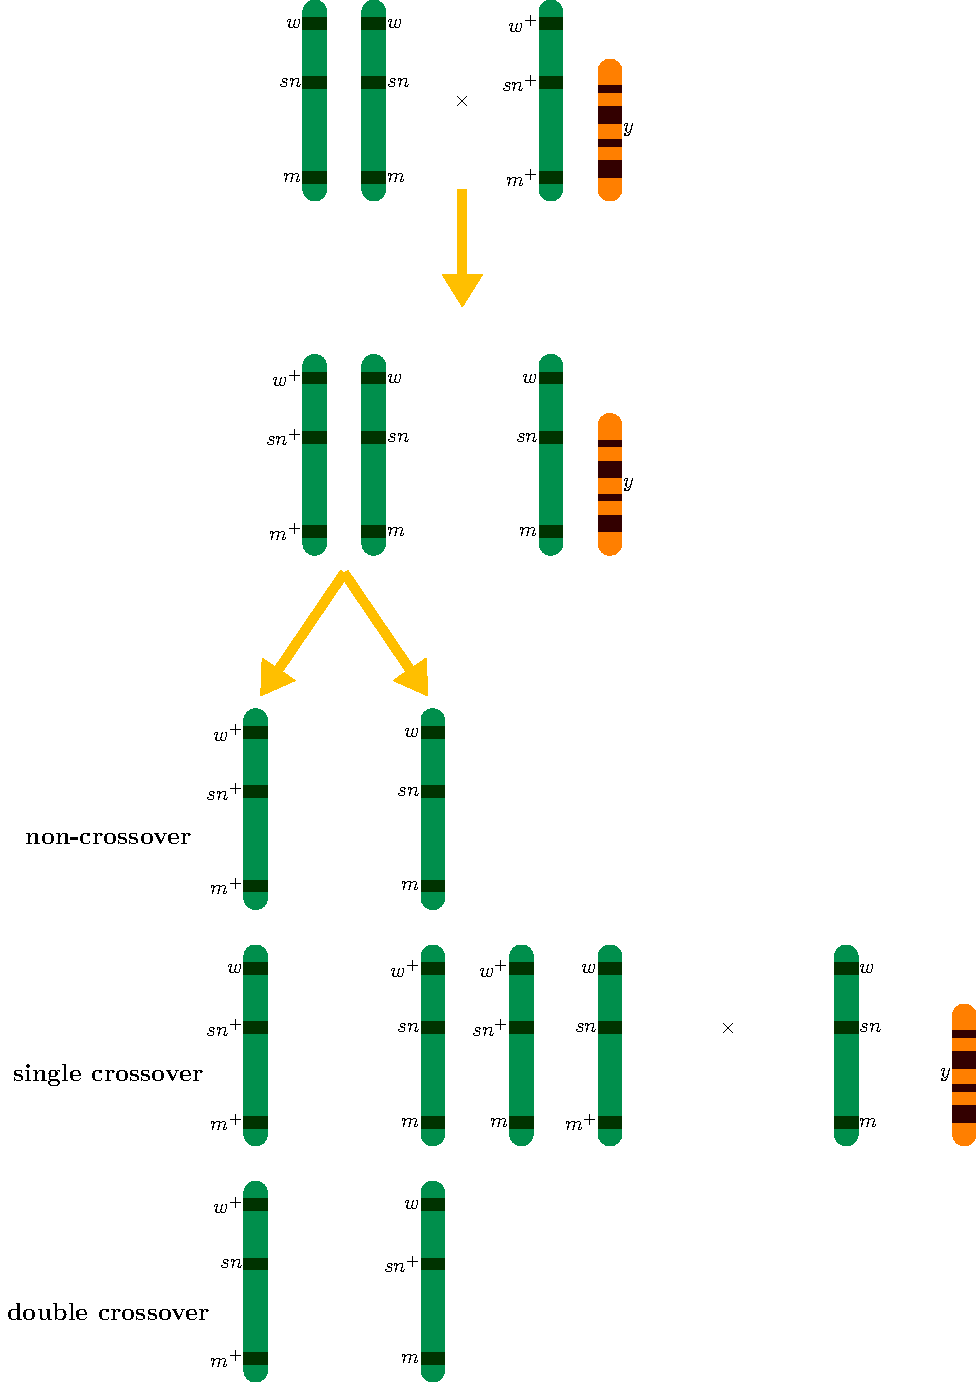
\includegraphics[height=0.45\textwidth]{draw/output/draw1.pdf}
        \label{fig:5-1}
    }
    \hfill
    \centering
    \subfloat[反交配子示意图]{
        \centering
        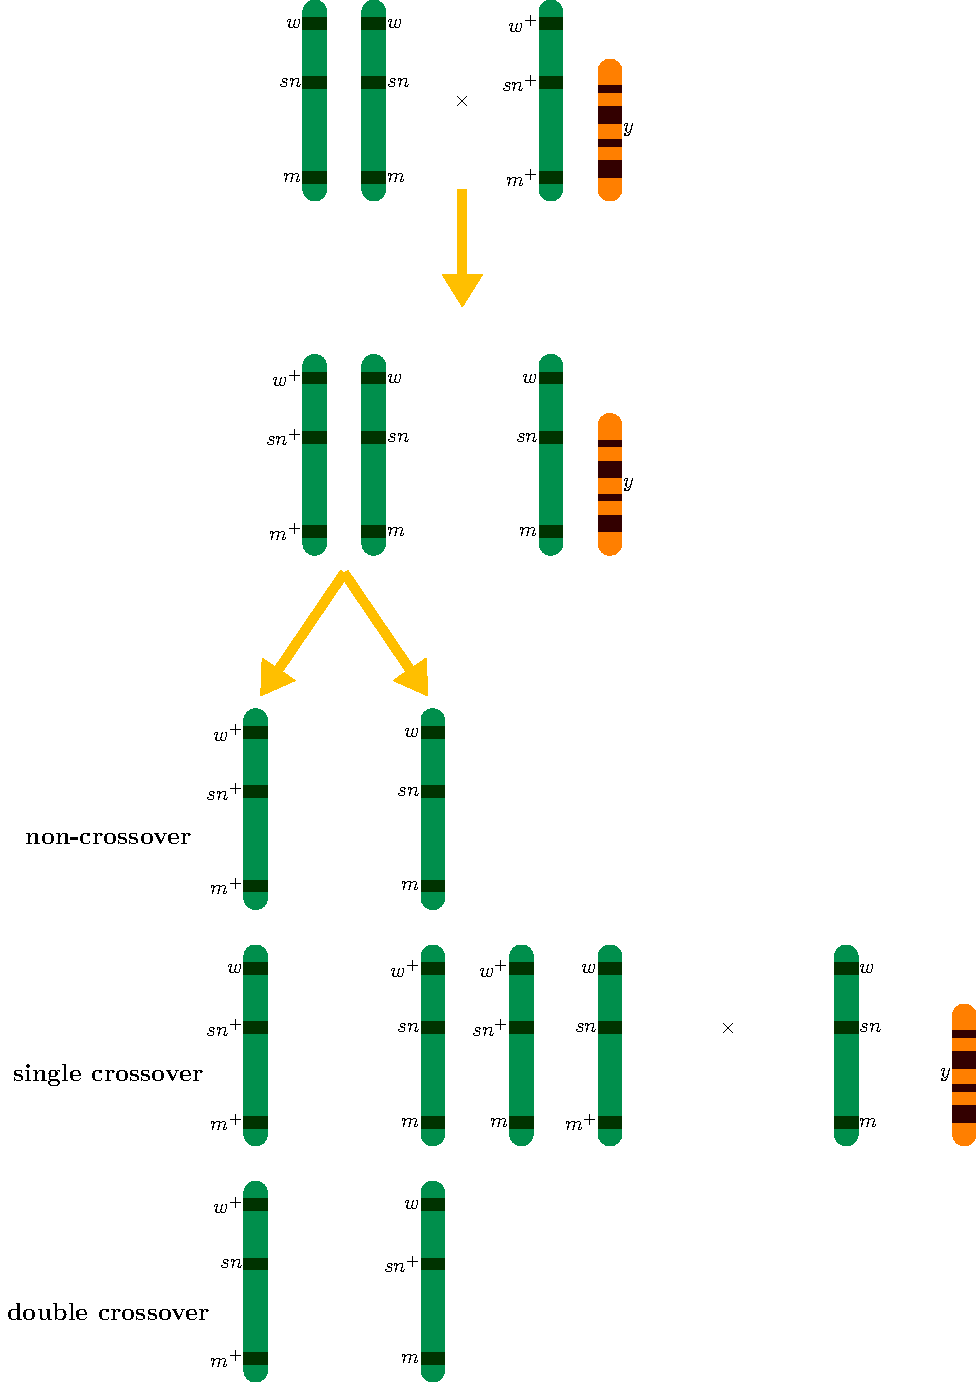
\includegraphics[height=0.45\textwidth]{draw/output/draw2.pdf}
        \label{fig:5-2}
    }
    \label{fig:5}
    \caption{正交和反交示意图}
\end{figure}

如图\ref{fig:5-1}, 在正交组合中, $F_1$代的雄性果蝇基因型为$w~sn~m//y$, 因此不论雄性果蝇的配子为$w~sn~m$还是$y$,
$F_2$中果蝇的表型都可以被表达出来, 相当于三点测交. 因此使用正交为对象可以相对正确的计算出图距和并发系数.
但是在反交组合中, 如图\ref{fig:5-2}, $F_1$代雄性果蝇基因型为$+~+~+//y$, 因此无论雌性的配子是什么, 
最终雌性后代的表现型都为红长直. 其中很多诸如单交换, 双交换的交换类型都无法被区分, 因此使用反交组合为对象计算出的图距和并发系数不准确.\par

总体而言,本研究通过果蝇的多因子遗传分析展示了遗传学三大定律在不同遗传组合下的表现,
揭示了基因之间的复杂相互关系。然而,需要注意的是,实验结果可能受到实验条件、样本数量等因素的影响,
存在一定的局限性。未来的研究可以进一步扩大样本量、深入挖掘基因之间的相互作用,
并探索新的遗传规律。这将有助于更全面地理解基因的遗传传递过程,为遗传学领域的发展提供更深入的见解。\par

需要注意的是, 我们在处理数据时发现, 本次实验的数据问题比较明显, 具体体现在$F_2$代反交雌性果蝇中, 
有很多组的数据中大量出现了本不该出现的除了红直长的其他表型, 在总共103组中, 其他表型出现的次数占全部次数不多于
30\%的组仅有64, 将这一占比降低至20\%后, 仅有29组数据符合要求. 根据3$\sigma$原则, 我们最终选择了30\%作为筛选的阈值. \par

虽说实验的结果大大不如预期, 但是同学们是第一次进行遗传学实验的新手, 在实验中锻炼并提高了自己的实验能力和技巧, 
克服了一个又一个难题, 也收获了一些经验, 为今后的实验打下了基础.\par

%论文后部
\backmatter


%=======%
%引入参考文献文件
%=======%
\bibdatabase{bib/database}%bib文件名称 仅修改bib/ 后部分
\printbib
%\nocite{*} %显示数据库中有的,但是正文没有引用的文献



\Appendix

点击打开\href{https://github.com/zehua0417/GeneticExperimentReport}{附录链接}

%\Thanks


%\Grade %这一句才是成绩页,上面是填写


\end{document}
